\chapter{Evaluating \where~on test data}% Main chapter title
\thispagestyle{nohead}
\label{Evaluation} 
%----------------------------------------------------------------------------------------

This chapter will evaluate the \where~SMT ranking predictions made on the held-back test data (see Sec. \ref{sub:train-test}).
The randomly-selected test set represents 25\% of the entire number of POs and consists of 32 WhyML files, 77 theories and 263 goals.
In addition to evaluating \where~'s \textit{predictions}, the OCaml implementation (detailed in the previous chapter) will be discussed in terms of its efficiency.   
We perform our evaluation guided by three Evaluation Criteria:
\begin{itemize}
	\item[EC1:] \textbf{How does \where~perform in comparison to the 8 SMT solvers?}\\
	The importance of this question is obvious: the success of \where~depends on its improvement over the status quo. In the case of discharging \why~POs, the status quo is represented as the use of a single solver.
	\item[EC2:] \textbf{How does \where~perform in comparison to the 3 theoretical strategies?}\\
	The theoretical strategies introduced in Sec. \ref{sec:strategies} provide a fairer basis for comparison than a single solver.
	\item[EC3:] \textbf{What is the time overhead of using \where~to prove \why~goals?}\\
	The feature extraction and solver scheduling processes incur a time cost. This criterion measures whether this cost represents a significant proportion of \where~'s overall solving time.    	
\end{itemize}
The chapter is organised around answering questions raised by each of the three criteria in turn.
The threats to the validity of our study are discussed in Sec. \ref{sec:threats}. 

\section{EC1: How does \where~perform in comparison to the 8 SMT solvers?}


\begin{table}
	\caption[Results for 8 solvers, \where~and 3 strategies on test set]{Number of files, theories and goals proved by each strategy and individual solver. The percentage this represents of the total 32 files, 77 theories and 263 goals and the average time are also shown.}
	\begin{tabularx}{1.1\textwidth}{@{}l|ZZZ|ZZZ|ZZZ@{}}
		\toprule
		{} & \multicolumn{3}{c|}{\textbf{File}} & \multicolumn{3}{c|}{\textbf{Theory}} & \multicolumn{3}{c}{\textbf{Goal}} \\
		{} & \# proved & \% proved & Avg time & \# proved & \% proved & Avg time & \# proved & \% proved & Avg time \\
		\midrule
		\where & 11 & 34.4\% & 1.75 &  44 & 57.1\% & 1.17 & 203 & 77.2\% & 2.10 \\
		\textsf{Best} & \downbar  & \downbar & 0.25 & \downbar & \downbar & 0.28 & \downbar & \downbar & 0.37 \\
		\textsf{Random} & \downbar & \downbar & 4.19 & \downbar & \downbar & 4.02 & \downbar & \downbar & 5.70 \\
		\textsf{Worst} & \upbar & \upbar & 14.71 & \upbar & \upbar & 13.58 & \upbar & \upbar & 18.35 \\
		%\textbf{\textsf{Where4} (tree)} & '' & '' & 4.08 & '' & '' & 2.52 & '' & '' & 3.50 \\
		\midrule
		\textbf{Alt-Ergo-0.95.2} & 8 & 25.0\% & 0.78 & 37 & 48.1\%& 0.26 & 164 & 62.4\% & 0.34 \\ 
		\textbf{Alt-Ergo-1.01} & 10 & 31.3\% & 1.07 & 39 & 50.6\% & 0.26 & 177 & 67.3\% & 0.33 \\ 
		\textbf{CVC3} & 5 & 15.6\% & 0.39 & 36 & 46.8\% & 0.21 & 167 & 63.5\% & 0.38 \\ 
		\textbf{CVC4} & 4  & 12.5\% & 0.56 & 32 & 41.6\% & 0.21 & 147 & 55.9\% & 0.35 \\ 
		\textbf{veriT} & 2 & 6.3\% & 0.12 & 24 & 31.2\% & 0.12 & 100 & 38.0\% & 0.27 \\ 
		\textbf{Yices} & 4 & 12.5\% & 0.32 & 32 & 41.6\% & 0.15 & 113 & 43.0\% & 0.18 \\ 
		\textbf{Z3-4.3.2} & 6 & 18.8\% & 0.46 & 31 & 40.3\% & 0.20 & 145 & 55.1\% & 0.37 \\ 
		\textbf{Z3-4.4.1} & 6 & 18.8\% & 0.56 & 31 & 40.3\% & 0.23 & 145 & 55.1\% & 0.38 \\ 
		\bottomrule
	\end{tabularx}
	\label{table:avgtimes2}
\end{table}

When each solver in \textsf{Where4}'s ranking sequence is run on each goal, the maximum amount of files, theories and goals are provable. 
As previously mentioned in Sec. \ref{sub:worst} and as Table \ref{table:avgtimes2} shows, the difference between \where~and the set of reference theoretical strategies (\textsf{Best}, \textsf{Random}, and \textsf{Worst}) is the amount of time taken to return the \textit{Valid/Invalid} result. 
Compared to the 8 SMT provers, the biggest increase is on individual goals: \textsf{Where4} can prove 203 goals, which is 26 (9.9\%) more goals than the next best single SMT solver, Alt-Ergo-1.01.

The average time \where~takes to prove these goals (following the sequential solving Algorithm \ref{algo:rank}) is significantly better than the \textsf{Random} strategy.
It is, however, lagging behind the time recorded by the \textsf{Best} strategy. 

In comparison to the 8 SMT provers, the average time taken by \where~to solve each of the 203 goals is high. 
This tells us that \where can perform badly with goals which are not provable by many SMT solvers: expensive \textit{Timeout} results are chosen before the \textit{Valid} result is eventually returned. 
In the worst case, \textsf{Where4} may try and time-out for all 8 solvers in sequence, whereas each individual solver does this just once. 
Thus, while having access to more solvers allows more goals to be proved, there is also a time penalty to portfolio-based solvers in these circumstances.

This raises the question of whether it fair to compare \where~to individual solvers. 
Any ranking strategy will be able to prove the maximum number of files, theories and goals, but unless the best solver is consistently placed first in the ranking, it could take a significantly longer time to do so than even the worst-performing individual solver.   

We remind the reader to the $\mathcal{TS}$ solver introduced in Sec. \ref{sec:portfolio-benefit}.
$\mathcal{TS}$ refers to the \textit{best single solver} as chosen on a per-goal basis.
It provided a motivation for the use of portfolio-solving on the \why~platform by proving the maximum number of goals in the shortest amount of time.
We mentioned that $\mathcal{TS}$ is equivalent to choosing  the top-ranking solver from \textsf{Best} and stopping.
We return to this concept in Fig. \ref{fig:barchart2} which is similar to Fig. \ref{fig:barcharts} in that it shows the relative amount of Valid/Unknown/Timeout/Failure answers from the eight SMT solvers. 
Also shown (on the right) are results obtainable by using the top solver (only) with the 3 ranking strategies (where \textsf{Best} $\equiv\mathcal{TS}$) and the \where~predicted ranking.

The 62 \text{Valid} answers returned by the solver from the \textsf{Worst} ranking (i.e. the worst solver) represent the trivial POs solvable by all 8 solvers. 
Likewise, the 60 goals for which \textsf{Best} did not return a \textit{Valid} or \textit{Invalid} answer could not be proved by any solver.

The results show that limiting the portfolio solver to just using the best predicted individual solver, eliminating the multiple time-out overhead yet reduces the number of goals provable by \where.
This number of goals -- 178 -- is still one more than the best-performing individual SMT solver, Alt-Ergo version 1.01.  

In an effort to compare \where~to individual SMT solvers, Table \ref{table:avgtimes2} and Fig. \ref{fig:barchart2} show results at two extremes of a spectrum: using all solvers available, and only using one.
In the next subsection we describe a method to calibrate the use of \where~by using cost predictions. 

\begin{figure}
	\centering
	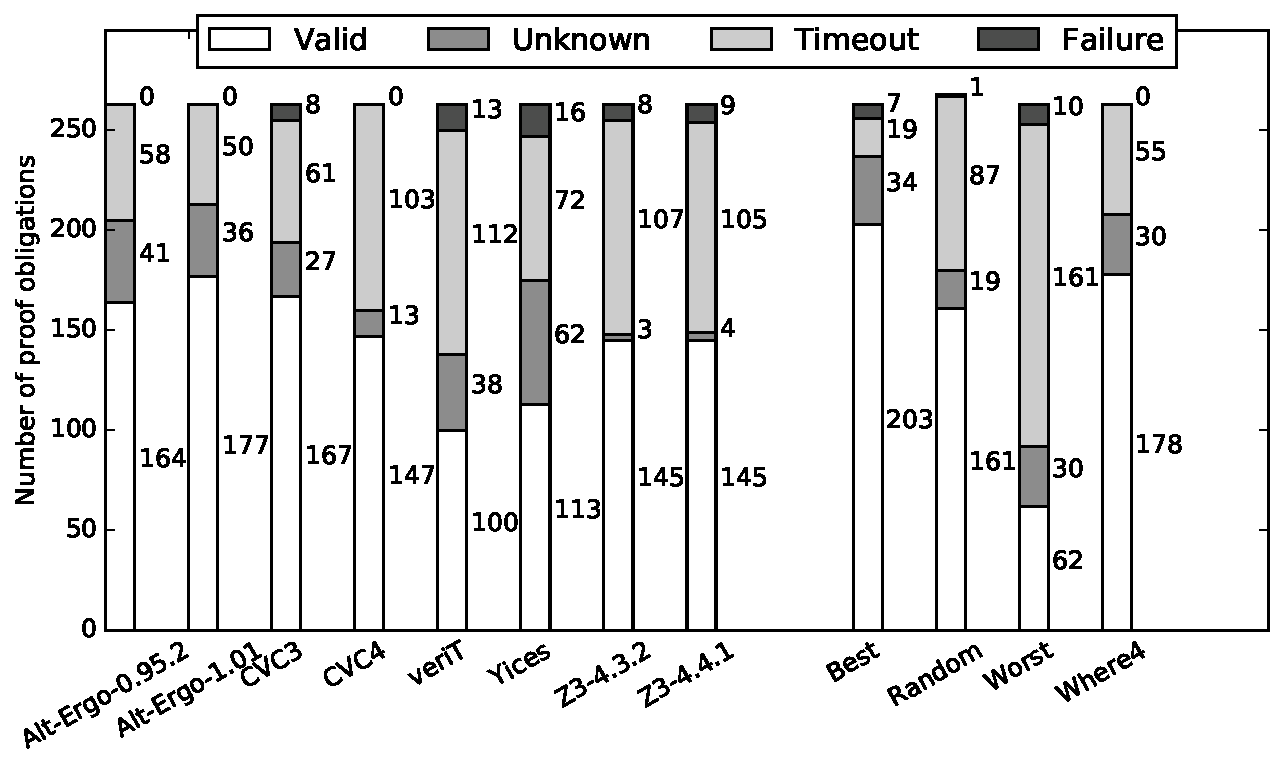
\includegraphics[width=\linewidth]{barcharts2}
	\caption[The relative amount of Valid/Unknown/Timeout/Failure answers from the eight SMT solvers, \where, and 3 theoretical strategies.]{The relative amount of Valid/Unknown/Timeout/Failure answers from the eight SMT solvers, \where, and 3 theoretical strategies.}
	\label{fig:barchart2}
\end{figure}

\subsection{Use of a cost threshold}

To calibrate the time-taken-versus-goals-proved trade-off associated with the two approaches above, we introduce the notion of a \textit{cost threshold} as another method of comparing \where~to individual SMT solvers.
Using this strategy, solvers with a predicted cost above this threshold are not called. 
If no solver's cost is predicted below the threshold, an \textit{Unknown} answer is returned instantly.
This modification to Algorithm \ref{algo:rank} is shown in Algorithm \ref{algo:threshold}    

\begin{algorithm}
	\caption{Returning answers and runtimes from \where~solver rankings using a cost threshold}
	\KwIn{$\langle$ Solver, cost $\rangle$ tuples  $ \lbrace \langle S_1, C_1 \rangle, ..., \langle S_n, C_n \rangle \rbrace$ sorted by predicted cost;\\
	$thresh$: the cost threshold}
	\KwOut{$\langle A,T\rangle$ where $A$ = the best answer from the solvers; $T$ = the cumulative time taken to return $A$}
	\Begin{
		\tcp{initialisation}
		$A \leftarrow Failure$ \\
		$T \leftarrow 0$ \\
		$i \leftarrow 1$ \\
		\If{$C_1 > thresh$ \tcp{No solver under the cost threshold} }
		{\Return{$\langle Unknown, 0\rangle$}}
		\While{$A \notin \lbrace Valid, Invalid \rbrace \wedge i \leq n \wedge C_i < thresh$}
		{$A_S \leftarrow Answer(S_i)$ \tcp{the answer returned by solver $S_i$
			}
			$T \leftarrow T + Time(S_i)$ \tcp{add solver $S_i$'s time to the cumulative runtime}
			\If{$A_S > A$}{$A \leftarrow A_S$ \tcp{$S_i$'s answer is better than the current best answer}}
			$i \leftarrow i + 1$}
		\Return{$\langle A,T\rangle$}} 
	\label{algo:threshold}
	
\end{algorithm}

\begin{figure}
	\centering
	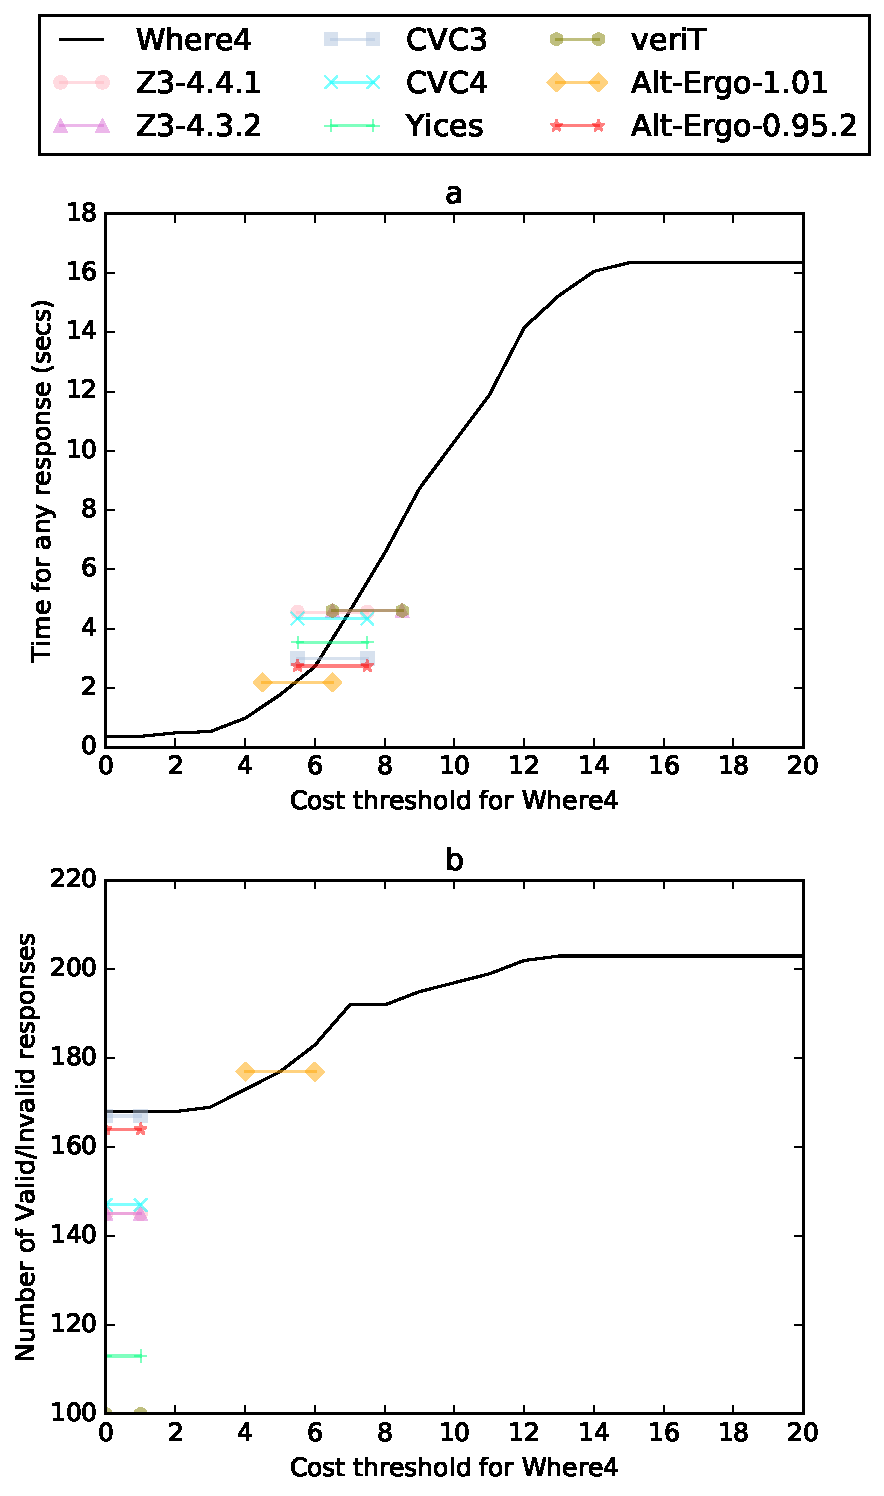
\includegraphics[width=\linewidth]{thresholds}
	\caption[The effect of using a cost threshold]{The effect of using a cost threshold. (\textit{black solid line -- left y axis}) The average time taken for \where~to return an answer compared to 8 SMT solvers. (\textit{cyan dashed line -- right y axis}) The number of Valid/Invalid answers returned by \where~compared to 8 SMT solvers.}
	\label{fig:thresholds}
\end{figure}

\begin{table}
	\caption[Results for 8 solvers, \where~and 3 strategies on test set]{Number of files, theories and goals proved by each strategy and individual solver. The percentage this represents of the total 32 files, 77 theories and 263 goals and the average time are also shown.}
	\begin{tabularx}{1.1\textwidth}{@{}l|ZZZ|ZZZ|ZZZ@{}}
		\toprule
		{} & \multicolumn{3}{c|}{\textbf{File}} & \multicolumn{3}{c|}{\textbf{Theory}} & \multicolumn{3}{c}{\textbf{Goal}} \\
		{} & \# proved & \% proved & Avg time & \# proved & \% proved & Avg time & \# proved & \% proved & Avg time \\
		\midrule
		\where & 11 & 34.4\% & 1.75 &  44 & 57.1\% & 1.17 & 203 & 77.2\% & 2.10 \\
		\textsf{Best} & \downbar  & \downbar & 0.25 & \downbar & \downbar & 0.28 & \downbar & \downbar & 0.37 \\
		\textsf{Random} & \downbar & \downbar & 4.19 & \downbar & \downbar & 4.02 & \downbar & \downbar & 5.70 \\
		\textsf{Worst} & \upbar & \upbar & 14.71 & \upbar & \upbar & 13.58 & \upbar & \upbar & 18.35 \\
		%\textbf{\textsf{Where4} (tree)} & '' & '' & 4.08 & '' & '' & 2.52 & '' & '' & 3.50 \\
		\midrule
		\textbf{Alt-Ergo-0.95.2} & 8 & 25.0\% & 0.78 & 37 & 48.1\%& 0.26 & 164 & 62.4\% & 0.34 \\ 
		\textbf{Alt-Ergo-1.01} & 10 & 31.3\% & 1.07 & 39 & 50.6\% & 0.26 & 177 & 67.3\% & 0.33 \\ 
		\textbf{CVC3} & 5 & 15.6\% & 0.39 & 36 & 46.8\% & 0.21 & 167 & 63.5\% & 0.38 \\ 
		\textbf{CVC4} & 4  & 12.5\% & 0.56 & 32 & 41.6\% & 0.21 & 147 & 55.9\% & 0.35 \\ 
		\textbf{veriT} & 2 & 6.3\% & 0.12 & 24 & 31.2\% & 0.12 & 100 & 38.0\% & 0.27 \\ 
		\textbf{Yices} & 4 & 12.5\% & 0.32 & 32 & 41.6\% & 0.15 & 113 & 43.0\% & 0.18 \\ 
		\textbf{Z3-4.3.2} & 6 & 18.8\% & 0.46 & 31 & 40.3\% & 0.20 & 145 & 55.1\% & 0.37 \\ 
		\textbf{Z3-4.4.1} & 6 & 18.8\% & 0.56 & 31 & 40.3\% & 0.23 & 145 & 55.1\% & 0.38 \\ 
		\bottomrule
	\end{tabularx}
	\label{table:threshold}
\end{table}


Fig. \ref{fig:thresholds} shows the effect of varying this threshold, expressed in terms of the average execution time (solid black line with its scale on the left $y$ axis) and the number of goals solved (dashed cyan line with its scale on the right $y$ axis).
As the corresponding results for each individual solver are unaffected by the threshold parameter, they are represented by horizontal line segments intersecting with the \where~data.
For added clarity, the Fig. \ref{fig:thresholds} data is presented in Tables \ref{} and \ref{}.
  
In choosing the best threshold parameter for \where, the $y$ value for the black solid line should be minimal -- meaning \textit{as low a value for time as practical} -- while the $y$ value for the dashed cyan line should be maximal -- meaning \textit{as many POs proved as practical}. 
Another way of looking at 
 
This graph emphasises how well Alt-Ergo 1.01 performs on the dataset: 

As we can see from both graphs in Fig. \ref{fig:thresholds}, for the goals in the test set a threshold of 7 for the cost function allows \textsf{Where4} to prove more goals than any single solver, in a time approximately equal to the four slower solvers (CVC4, veriT and both versions of Z3). 



\section{EC2: How does \where~perform in comparison to the 3 theoretical strategies?}

\section{EC3: What is the time overhead of using \where~to prove \why~goals?}

\section{Threats to Validity}
\label{sec:threats}
\subsection{Internal}
\subsection{External}


\section{Discussion}